\section{Implementacja}

\begin{frame}
	\frametitle{Proces kompilacji}

	\begin{columns}
		\begin{column}{0.5\textwidth}
			\begin{itemize}
				\item Kod użytkownika musi być wykonywany w czasie kompilacji
				\item Reprezentacja pośrednia programu musi być wtedy dostępna
				\item Część kompilatora może zostać napisana w języku docelowym
			\end{itemize}
		\end{column}
		\begin{column}{0.5\textwidth}  %%<--- here
			\begin{center}
			 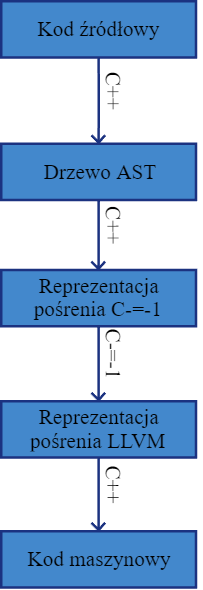
\includegraphics[height=6cm]{../assets/toplevelcompilationprocess.png}
			 \end{center}
		\end{column}
	\end{columns}
\end{frame}

\begin{frame}
	\frametitle{Proces kompilacji}

	\begin{itemize}
		\item Kod użytkownika musi być wykonywany w czasie kompilacji
		\item Reprezentacja pośrednia programu musi być wtedy dostępna
		\item Część kompilatora może zostać napisana w języku docelowym
		\item Kompilator jest bliższy interpreterowi Pythona niż gcc
	\end{itemize}

\end{frame}

\begin{frame}
	\frametitle{Kompilacja przez interpretację}

	\begin{figure}
		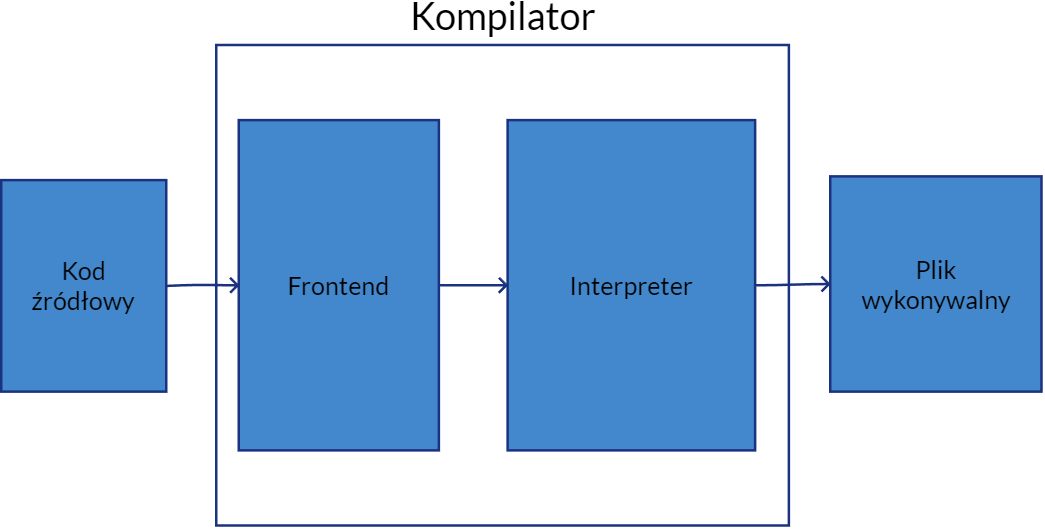
\includegraphics[width=\textwidth]{../assets/compilerouterdiagram.png}
	\end{figure}

\end{frame}

\begin{frame}
	\frametitle{Kompilacja przez interpretację}

	\begin{itemize}
		\item Budowana jest reprezentacja pośrednia programu.
		\item Komponent kompilujący do kodu maszynowego jest napisany w języku docelowym i jest interpretowany.
		\item Interpreter udostępnia narzędzia do budowy kodu maszynowego
		\item Komponent kompilujący może być wymieniany przez użytkownika
	\end{itemize}

\end{frame}

